% Vorlesung 1.9.19

\chapter{Grundlagen der Quantenmechanik}

\lcom{Dies ist das letzte Kapitel dieser Vorlesung. Vektor Algebra muss man für dieses Kapitel gut verstanden haben.}

\section{Axiome der Quantenmechanik}

\folie{Die Axiome der Quantenmechanik}
\begin{enumerate}[I)]
	\item Der Zustand wird beschrieben durch die Wellenfunktion $ \Psi $ bzw. den Zustandvektor $ |\Psi \rangle $\\
	$$ \Psi = \tx{ Wellenfunktion}$$
	$$ \vert\Psi\rangle = \tx{ Zustandsvektor, q.m. Zustand, Zustand}$$
	\item Einer Messbaren Eigenschaft ist ein hermitescher Operator $ \hat{A} $ zugeordnet, $ \hat{A} $ heißt Observable\\
	Impuls $\leftrightarrow$ $\vec{\hat p}$ = $\begin{pmatrix} \hat p_x \\ \hat p_y \\ \hat p_z \end{pmatrix}$\\
	Ort $\leftrightarrow\ \vec{\hat x}$\\
	Energie $\leftrightarrow\ \hat H$
	\item Der Erwartungswert eines Operators $ \hat{O} $ im Zustand $ |\Psi\rangle $ bzw. für die Wellenfunktion $ \Psi $ ist gegeben durch:
	 $ \langle \hat{ O \rangle} = (\Psi, \hat{O}, \Psi) \quad $ oder $ \quad \langle \hat O \rangle = \langle \Psi \vert \color{black!20!red}\hat O \color{black}\vert \color{black!30!green} \Psi \color{black}\rangle = \sum_n \overbrace{\color{black!30!green}p_n}^{\mathclap{\tx{Wahrscheinlichkeit}}} \underbrace{\color{black!20!red}a_n}_{\mathclap{\tx{Zahlen}}}$\\
	Wobei das erste $\langle \hat O \rangle$ das statistische Mittelwert bedeutet. \\
	\lcom{Diese aussage gilt für alle Operatoren, nicht nur Hermitesche.}
	\item Die Zeitentwicklung der Zustände bzw. Wellenfunktionen wird durch die Schrödinger-Gleichung beschrieben:\\
	DGL $\overbrace{\prt{}{t}}^{\tx{1. ord}}$
	\item Bei Messungen der Observablen $ \hat{A} $ für ein System im Zustand $ |\Psi \rangle $ bzw. der Wellenfunktion $ \Psi $ erhält man mit der Wahrscheinlichkeit $ p_n = |\Psi_n, \Psi)|^2 $ bzw. $ p_n = |\langle \Psi_n | \Psi \rangle |^2 $ den Eigenwert $ a_n : $ der Zustand des Systems geht in die zugeorsnete Eigenfunktion $ \Psi_n $ bzw. $ |\Psi_n\rangle $ über (Messprozess $ \rightarrow $ Kollaps der Wellenfunktion).
\end{enumerate}
Außerdem gilt: Der Erwartungswert $ \langle \hat{A} \rangle $ der Observablen $ \hat{A} $ ist der Mittelwert der Messergebnisse $ a_n $ von sehr vielen (gleichen) Experimenten $ \langle \hat{A} \rangle = \sum_n p_n a_n $.

\section{Wellenfunktion, Operatoren, Zustände}

\subsection{Wellenfunktionen}

\subsubsection{Doppelspalt}

\folie{Interferenz/Einzel-Teilchen Experimente}\\
$$\vec{E}\tx{: relle, vektorielle Funktion um }\vec{r}\tx{ und }t$$
$$\Psi\tx{: komplexe, skalare Funktion von } \vec{r} \tx{ und }t$$

\subsubsection{Interpretation der Wellenfunktion}

$|\Psi(\vec{r},t)|^2$ ist die Wahrscheinlichkeit dafür ein Teilchen zur Zeit $t$ am Ort $\vec{r}$ zu finden.\\

\subsubsection{$\Rightarrow$ Normierung}

Gesamtwahrscheinlichkeit muß 1 sein. $\Rightarrow\ \int \Psi^*(\vec{r},t) \Psi(\vec{r},t) \dd \vec{r} = 1$ wobei $\Psi^*$ das komplex konjugierte ist.

\subsection{Operatoren}

\lcom{Die mathematische Definition ist fürchterlich einfach.}

\subsubsection{Mathematische Definition}

$$\Psi' = \hat O \Psi \qquad |\Psi'\rangle = \hat O | \Psi \rangle$$

\subsubsection{Anschauliche Definition}

Ein Operator verändert einen Zustand.\\
\bei
$$\Psi'(\vec{r},t) = C e^{\frac{i}{\hbar} (\vec{p} \cdot \vec{r} - Et)}$$
\begin{itemize}
	\item $\hat O = (5 + 3i) \qquad \Psi'(\vec{r}, t) = (5 + 3i) \Psi(\vec{r},t) = (5 +3i)C e^{\frac{i}{\hbar}(\vec{p}\vec{r}- Et)}$
	\item $\hat O = \prt{}{t} \qquad \Psi'(\vec{r}, t) = \prt{}{t}\Psi(\vec{r},t) = -C\frac{i}{\hbar}E e^{\frac{i}{\hbar}(\vec{p}\vec{r}- Et)}$
	\item $\hat O = \prt{}{x} \qquad \Psi'(\vec{r}, t) = \prt{}{x} \Psi(\vec{r},t) = C\frac{i}{\hbar}p_x e^{\frac{i}{\hbar}(\vec{p}\vec{r}- Et)}$
	\item $\hat O = \tx{Zeitumkehroperator}:\ \hat T \qquad \Psi'(\vec{r}, t) = \hat T \Psi(\vec{r},t) = \Psi(\vec{r},-t)$
\end{itemize}
\subsection{Hilbert-Raum (Ultrakompakt)}
Frage: Was ist der Unterschied bzw. Zusammenhang zwischen $\Psi$ und $|\Psi\rangle$???\\
Antwort:
\rbox{$\Psi(\vec{r},t)$ ist die Wellenfunktion des Zustandes $|\Psi(\vec{r},t)\rangle$ in der Ortsdarstellung.}
\subsubsection{Vektorraum}
$$\vec{v}(t) = \sum_k c_k (t) \vec{e}_k$$
$\custo{\rightarrow}{\tx{Vektor}}{\ |\Psi\rangle}$ = $\custo{\rightarrow}{\tx{Koordinaten}}{\ \Psi}$ und $\custo{\rightarrow}{\tx{Basisvektoren}}{\tx{Darstellung}}$ (Koordinatensystem) 

\subsubsection{Reihenentwicklung von Funktionen, Funktionen als Vektorraum}

\begin{equation*}
f(x) = \sum_{k} c_k g_k(x) \qquad \tx{diskreten}
\end{equation*}
\begin{equation*}
\tx{Funktion } = \tx{ Entwicklungskoeffizienten } \& \tx{ Funktionenbasis}
\end{equation*}
\begin{enumerate}[(1)]
	\item endlich diskret
	\begin{equation*}
	f(x) = \sum_{k=0}^{N} c_k g_k(x)
	\end{equation*}
	\item unendlich diskret
	\begin{equation*}
	f(x) = \sum_{k=0}^{\infty} c_k g_k(x)
	\end{equation*}
	\item kontinuierlich
	\begin{equation*}
	f(x) = \int c(k) g(k,x) \dd k
	\end{equation*}
	\item diskret + kontinuierlich
	\begin{equation*}
	f(x) = \sum_{k} c_k g_k(x) + \int c(k) g(k,x) \dd k
	\end{equation*}
\end{enumerate}
\emph{Beispiele:}
\begin{itemize}
	\item Fourier-Reihe: unendlich diskret
	\begin{equation*}
	f(x) = \frac{a_0}{2} + \sum_k a_n \cos(n \omega_0 t) + b_n \sin(n \omega_0 t)
	\end{equation*}
	\item Fourier-Integral/Transformation: kontinuierlich
	\begin{equation*}
	f(x) = \int F(\omega) e^{-i \omega t} \dd \omega
	\end{equation*}
	$ e^{-i \omega t} : $ Basisfunktionen\\
	$ F(\omega) : $ Entwicklungskoeffizienten
	\item Kugelflächenfunktionen:
	\begin{equation*}
	f(0,1) = \sum_{l = 0} \sum_{m = -l}^{l} c_{lm} Y_{m}^{l}(0,1)
	\end{equation*}
	\item Taylor-Reihe:
	\begin{equation*}
	f(x) = \sum_n \frac{1}{n !} f^{(n)} (0) x^n
	\end{equation*}
	\item Legendre-Polynome:
	\begin{equation*}
	f(x) = \sum_n c_n P_n(x)
	\end{equation*}
\end{itemize}
\lcom{Sehr allgemeines Konzept, es gibt viele Beispiele wie Hermitesche Polynome.}

\subsubsection{Hilbertraum}

Ähnlich wie ein Vektorraum, nur mit Funktionen als Basis.
\begin{equation*}
\tx{Funktionsbasis } + \tx{ gewisse Eigenschaften}
\end{equation*}

\subsubsection{Bracket-Notation}

\begin{equation*}
|\custo{\leftarrow}{\quad}{\mathclap{\tx{Freiraum}}} \rangle
\end{equation*}
\begin{equation*}
|\Psi\rangle , |\vec{r}, t \rangle , | \Psi, t \rangle , | n \rangle , | E \rangle , | \dots \rangle
\end{equation*}
\lcom{die Bracket können vieles bedeuten wie zum Beispiel $f(x)$ kann alle möglichen Funktionen darstellen.}

\subsection{Zustand Darstellung und Wellenfunktion}

\begin{alignat*}{3}
&|\Psi\rangle = &&\Psi \qquad \tx{und} &&| n\rangle\\
&\tx{Zustand}\quad &&\tx{Wellenfunktion}\quad &&\tx{Darstellung}\\
&\vec{v} = &&\tx{Koordinaten} &&\tx{Basisvektoren}
\end{alignat*}

% hier ein bisschen misst der so gesagt wurde und dann aus dem kontext genommen wurde
\begin{comment}
\chapter{Der Liebe Gott}
\section{Verliebt sein}
\subsection{wer darf wo rumfumeln}
rumfumeln ist nicht unabhängig
\subsection{was gehört zu wem}
\section{Gender-Theorie}
es gibt unendliche viele Wahrscheinlichkeiten und Zuordnungen (von Gendern)
\section{Der Satz von Stinson}
\end{comment}

% Vorlesung 15.01.18


% andrez:
% 1.15.19
%
%\bbb{Wiederholung}{QM}
%
\noindent
Darstellungswechsel: $\widehat =$ Koordinatentransformations/Basiswechsel
\bei 
\begin{itemize} 
	\item Ortsdarstellung: Basis sind die Ortseigenfunktionen $|\vec{r}\rangle$
	$$\vec{\hat r} | \vec{r} \rangle = \vec{r}| \vec{r}\rangle$$
	$$\Rightarrow |\Psi, t\rangle =\int \underbrace{\Psi(\vec{r},t)}_{\mathclap{\tx{Wellenfkt. in Ortsdarstellung}}}|\vec{r}\rangle \dif\vec{r}$$
	\item Impulsdarstellung: Basis sind die Impulsdeigenfunktion $|\vec{p}\rangle$
	$$\vec{\hat p} |\vec{p} \rangle = \vec{p} | \vec{p}\rangle$$
	$$\Rightarrow |\Psi, t \rangle =\int \underbrace{\Psi(\vec{p},t)}_{\mathclap{\tx{Wellenfkt. in Impulsdarstellung}}}|\vec{p}\rangle$$
	\item Energie- (Spektral-) Darstellung: Basis sind Energieeignefunktionen $|E_n \rangle$
	$$\hat \ham| E_n\rangle = E_n|E_n\rangle$$
	$$\Rightarrow |\Psi,t\rangle =\sum_k \underbrace{C_k (t)}_{\substack{ \\[5pt] \mathclap{\tx{Wellenfkt. in der Energiedarstellung}}}} |E_n\rangle$$
\end{itemize}

\subsection{Analogie zwischen Vektor- und Hilbertraum}
$$\vec{v}(t) = \sum_k C_k (t) \vec{e}_k \qquad \leftrightarrow \qquad |\Psi,t\rangle = \sum_n C_n (t) |n\rangle \quad \tx{oder} \quad |\Psi,t\rangle = \int C(n,t)|n\rangle\dif n$$
\folie{Analogie zwischen Vektor- und Hilbertraum}

\subsubsection{Vektoroperator}
$$\vec{p} = \begin{pmatrix} p_x \\ p_y \\ p_z \end{pmatrix} \hat = \mathop{} \vec{\hat p} = \begin{pmatrix}\hat p_x \\ \hat p_y \\ \hat p_z \end{pmatrix}$$
\lcom{Wir brauchen alle drei Zahlen um die Bewegung des Teilchens zu beschreiben.}
\section{Nicht relativistische QM und Schrödingergleichung}
\subsection{Zustand und Bewegung eines Teilchens}

klassisch:
\begin{description}
	\item[Zustand] $\vec{v}(t), \vec{p}, t$
	\item[Messgrößen] können ausgedrückt werden als Funktionen um $\vec{v}(t), \vec{p}(t),t, \dots$
	\item[Bewegung] Hamiltonfunktion $\ham(\vec{r},\vec{p}) = E$
\end{description}
QM, in der Sprache der Wellenfunktionen in der Ortsdarstellung
\begin{description}
	\item[Zustand] Wellenfunktion $\Psi(\vec{r},t)$
	\item[Messgrößen] Eigenwert $a_k$ der Observable $\hat A$ mit einer Wahrscheinlichkeit $p_k = |(\Psi_k, \Psi)|^2$
	\item[Bewegung] Hamiltonoperator $\hat \ham(\vec{\hat r},\vec{\hat p})$
	$$i \hbar \prt{}{t} \Psi(\vec{r}, t) = \hat \ham \Psi(\vec{r}, t)$$
\end{description}
QM in der Sprache der Zustandsfunktionen
\begin{description}
	\item[Zustand] $|\Psi,t\rangle$
	\item[Messgrößen] Eigenwert $a_k$ der Observable $\hat A$ mit einer Wahrscheinlichkeit $p_k = |\langle\Psi_k | \Psi\rangle|^2$
	\item[Bewegung] $$i \hbar \prt{}{t} | \Psi(\vec{r}, t) \rangle = \hat \ham |\Psi,t\rangle$$
\end{description}
$ \rmbox{\vec{F} = m \vec{a}} $

\subsubsection{Wichtige Darstellung}

\begin{itemize}
	\item $t$ ist ein Parameter
	\item $\vec{r}$ in $\Psi(\vec{r},t)$ hängt nicht implizit selber um $t$ ab.
	\item $\vec{r}$ in $\Psi(\vec{r},t)$ ist \color{red} NICHT \color{black} der Ort des Teilchens \mau\\
	Der Ort der Teilchens ergibt sich aus Axiom V)
	$$p(\vec{r}) = |(\Psi_{\vec{r}}|\Psi)|^2 = |\Psi(\vec{r},t)|^2$$
	\item $\Psi(\vec{r},t)$ hängt \color{red} NUR \color{black} von $\vec{r}$ und $t$ ab, \color{red} NICHT \color{black} von z.B. $\vec{p}, E, \dots$\\
	Der Impuls des Teilchens ergibt sich aus Axiom V)
	$$p(\vec{p}) = |(\Psi_p | \Psi)|^2 = \cancel{| \Psi(p,t)|^2}$$
\end{itemize}

%markus:
\subsection{,,Herleitung`` der Schrödingergleichung (SGL)}

Wir betrachten ein freies Teilchen $ \widehat{=} $ Ebene Welle $ \quad \Psi(\vec{r},t) = C e^{\frac{i}{\hbar} (\vec{p} \cdot \vec{r} - E t)} $

\subsubsection{Ortsoperator}

\begin{equation*}
\hat{\vec{r}} \Psi = \vec{r} \Psi \quad \tx{ nach Konstanten}
\end{equation*}

\subsubsection{Impulsoperator}

\begin{equation*}
\hat{\vec{p}} \Psi = \vec{p} \Psi
\end{equation*}
Beobachte: $ \prt{}{x} \Psi = \frac{i}{\hbar} p_x \Psi \quad \Rightarrow \quad \vabla \Psi = \frac{i}{\hbar} \vec{p} \Psi $
\begin{equation*}
\Rightarrow \quad \rmbox{\hat{\vec{p}} = - i \hbar \vabla} \quad \tx{ Impulsoperator in der Ortsdarstellung}
\end{equation*}

\subsubsection{Schrödinger-Gleichung}

\begin{equation*}
\hat{E} \Psi = E \Psi
\end{equation*}
Beobachte: $ \prt{}{t} \Psi = - \frac{i}{\hbar} E \Psi $
\begin{equation*}
\Rightarrow \quad \rmbox{\hat{E} = i \hbar \prt{}{t}}
\end{equation*}
Neben klassischer Gleichung $ \ham(\vec{r},\vec{p}) = E $, und ersetzen durch Operatoren
\begin{equation*}
\rmbox{i \hbar \prt{}{t} \Psi(\vec{r},t) = \hat{\ham}(\hat{\vec{r}}, \hat{\vec{p}}) \Psi(\vec{r},t)}
\end{equation*}
$ \Rightarrow $ Verallgemeinerung: Zeitabhängige Schrödinger-Gleichung
\frbox{Zeitabhängige Schrödinger-Gleichung}{
\begin{equation*}
i \hbar \prt{}{t} |\Psi,t\rangle = \hat{\ham} (\hat{\vec{r}}, \hat{\vec{p}}) |\Psi,t\rangle
\end{equation*}
}

\subsection{Freies Teilchen in Ortsdarstellung}

klassisch:
\begin{equation*}
\ham (\vec{r}, \vec{p}) = \frac{\vec{p^2}}{2 m}
\end{equation*}
quantenmechanisch:
\begin{equation*}
\hat{\ham} = \frac{\hat{\vec{p}}^2}{2 m} = - \frac{\hbar^2}{2 m} \vabla^2 \qquad (\vabla^2 = \prt{^2}{x^2} + \prt{^2}{y^2} + \prt{^2}{z^2} = \Delta)
\end{equation*}
da $ \hat{\vec{p}} = - i \hbar \vabla $\\[5pt]
Schrödingergleichung:
\begin{equation*}
i \hbar \prt{}{t} \Psi(\vec{r},t) = - \frac{\hbar^2}{2 m} \vabla^2 \Psi(\vec{r},t)
\end{equation*}
\textbf{Lösung:}
\begin{enumerate}[i)]
	\item Lösungsansatz:
	\begin{equation*}
	\Psi(\vec{r},t) = Ce^{\frac{i}{\hbar} (\vec{p} \cdot \vec{r} - E t)}
	\end{equation*}
	\item 1. Seite der Schrödinger-Gleichung: $ \quad i \hbar \prt{}{t} \Psi = E \Psi $
	\item 2. Seite der Schrödinger-Gleichung: $ \quad -\frac{\hbar^2}{2 m} \left(\frac{i}{\hbar} \vec{p}\right)^2 \Psi = \frac{\vec{p}^2}{2 m} \Psi $
	\begin{equation*}
	\Rightarrow \quad E \cancel{\Psi} = \frac{\vec{p}^2}{2 m} \cancel{\Psi}
	\end{equation*}
	\begin{equation*}
	\rmbox{E = \frac{\vec{p}^2}{2 m}} \quad \checkmark \qquad \Rightarrow \quad \Psi(\vec{r},t) = C e^{\frac{i}{\hbar} (\vec{p} \cdot \vec{r} - E t)}
	\end{equation*}
\end{enumerate}

\subsection{Teilchen im Potential in Ortsdarstellung}

klassisch:
\begin{equation*}
\ham(\vec{r},\vec{p}) = \frac{\vec{p}^2}{2 m} + V(\vec{r})
\end{equation*}
quantenmechanisch:
\begin{equation*}
\hat{\ham} = - \frac{\hbar^2}{2 m} \vabla^2 + V(\vec{r})
\end{equation*}
Schrödinger-Gleichung:
\begin{equation*}
i \hbar \prt{}{t} \Psi(\vec{r},t) = \left(- \frac{\hbar^2}{2 m} \vabla^2 + V(\vec{r})\right) \Psi(\vec{r},t)
\end{equation*}
\emph{Bemerkung:}
\begin{itemize}
	\item ebene Wellen sind \textbf{keine Lösung} dieser SGL
	\begin{equation*}
	\Psi = \tx{ ebene Welle} \quad \Rightarrow \quad E = \frac{\vec{p}^2}{2 m} + V(\vec{r}) \qquad \tx{weil in Ortsdarstellung gilt: } \quad \hat{\vec{r}} \Psi = \vec{r} \Psi 
	\end{equation*}
	\LARGE{\lightning} \normalsize $ E \neq \const : \quad E(\vec{r}) $\\
	Wir wissen aber $ E $ ist nicht vom Ort abhängig sondern eine Konstante.\\
	Hier ist der Lösungsansatz also Falsch. \LARGE{\lightning} \normalsize
\end{itemize}

\subsection{Zeitunabhängige SGL}

Für explizit nicht von der Zeit abhängiger Hamiltonoperatoren läßt sich die SGL allgemein lösen:\\[5pt]
Ansatz:
\begin{equation*}
|\Psi,t\rangle = f(t) |\Psi,0\rangle
\end{equation*}
$ \Rightarrow $ in zeitabhängige SGL einsetzen $ \Rightarrow $ Gleichung separieren $ \Rightarrow $ zwei Gleichungen für die zwei separierten Bruchstücke
\begin{enumerate}[(1)]
	\item eine Lösung stellt sich als eindeutig heraus
	$$ f(t) = e^{-\frac{i}{\hbar} Et} $$
	\item$ \phantom{0} $\\[-30pt]
	\frbox{Zeitunabhängige Schrödinger-Gleichung}{
	\begin{equation*}
	\hat{\ham} |\Psi,0\rangle = E |\Psi,0\rangle
	\end{equation*}
	}
\end{enumerate}
\textbf{Feststellung 1:}
\begin{equation*}
\rmbox{\tx{Das ist eine Eigenwertgleichung zum Hamiltonoperator}}
\end{equation*}
\begin{equation*}
\begin{array}{l|l}
	\tx{diskret} & \tx{kontinuierlich}\\
	\hline\\[-5pt]
	\hat{\ham} |n\rangle = E_n |n\rangle & \hat{\ham} |n\rangle = E(n) |n\rangle\\
\end{array}
\end{equation*}
$ n $ abzählbar\\[5pt]
\textbf{Feststellung 2}\\
Die Lösungen sind die stationären Zustände des Quantensystems\\[5pt]
\textbf{Feststellung 3}\\
F1 ist äquivalent zu F2\\[10pt]

% Vorlesung 16.01.18

%andrez:
\bbb{Wiederholung}{Ansatz: $$|\Psi,t\rangle = f(t)|\Psi,0\rangle$$
	1) $f(t) = e^{-\frac{i}{\hbar} Et}$\\
	2) $ \hat \ham |\Psi,0\rangle = E|\Psi,0\rangle$\\
	Festellung 2:
	$$\langle \hat O \rangle(t) = \tx{mit unabhängig für stationäre zustände}$$}

\subsection{Zusammenfassung}

\begin{description}
	\item[Zustand, Wellenfunktion, Darstellung] $|\Psi\rangle = \sum_k \Psi_k|k\rangle$ oder $|\Psi\rangle = \int \Psi(k)|k\rangle \dif k$
	\item[Operatoren] $\Psi' = \hat O \Psi, \quad |\Psi'\rangle = \hat O| \Psi\rangle$
	\item[Messung] Axiom V
	\item[Bewegung] const. $i\hbar \prt{}{t}|\Psi,t\rangle = \hat \ham |\Psi,t\rangle$
	$$+ \prt{}{t}\hat \ham = 0 \quad E|\Psi\rangle = \hat \ham|\Psi\rangle, \quad |\Psi,t\rangle = e^{\frac{i}{\hbar}Et}|\Psi\rangle$$
\end{description}

\section{Stern-Gerlach Experiment und Elektronen-Spin (1922 - 25)}

Ziel: Messung des magnetischen Moments $\vec{\mu}$ von Atomen
$$\vec{\tau} = \vec{\mu} \times \vec{B}$$
\lcom{In einem inhmogenen Magnetfeld gibt es einen Feldgradienten undgleich null und damit eine Faraday-Kraft:}\\
Faraday Kraft $\vec{F} = \vec{\nabla}(\vec{\mu}\cdot\vec{B})$\\[5pt]
\begin{minipage}{.75\linewidth}
	\textbf{Vorbereitung:}\\[5pt]
	$\vec{L} = \vec{v} + \vec{p}$\\
	$\vec{\mu} = IA \vec{n}$
	$$\Rightarrow \quad \rmbox{\vec{\mu} = \frac{q}{2m}\vec{L}}\quad \tx{Klassisch}$$
\end{minipage}%
\begin{minipage}{.25\linewidth}
	\flushright
	%t1 :
	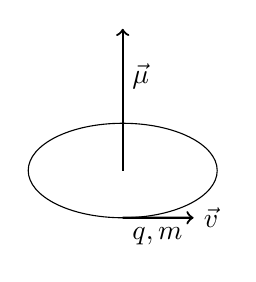
\begin{tikzpicture}[scale=.6]
		\draw[thick, ->] (0,0) -- (0,3);
		\draw (0,0) ellipse(2cm and 1cm);
		\coordinate (a) at (0,-1);
		\node[right] at (0,2) {$\vec{\mu}$};
		\node[anchor=north west] at (a) {$q,m$};
		\draw[thick,->] (a) -- (1.5,-1) node[right] {$\vec{v}$};
	\end{tikzpicture}
\end{minipage}%

\subsubsection{Aufbau und Durchführung}

Klassische Erwartung % $$\vec{\mu}$$: vermutlich nichts:
$$\vec{F} = \vec{\nabla}(\vec{\mu} \cdot \vec{B}) = \underbrace{\mu_z}_{\mathclap{\color{red}\tx{wird gemessen}}} \prt{B}{z} \vec{e}_z$$
Ofen $\Rightarrow$ statische Verteilung der Richtungen des $\vec{\mu}$'s der Atome

\subsubsection{Experiment}

\folie{The Spin, A Quantum Magnet (video)}\\[10pt]
\versuch{Magnetische Dipole durch inhomogenes Feld}
$ \Rightarrow $ nur zwei arten von Dipolen werden gemessen $ \pm p_z $, da nur $ p_z $ gemessen wird.\\
So als würden nur Dipole mt zwei verschiedenen Richtungen in das inhomogene Magnetfeld eintreten. Wir wissen aber, dass die eintretenden Dipole in \textbf{alle Richtungen} zeigen.\\[10pt]
Schlussfolgerungen:
\begin{enumerate}[1)]
	\item Das Elektron trägt neben der Ladung zusätzlich ein magnetisches Moment $ \vec{\mu}_e $.
	\begin{equation*}
	\Rightarrow \quad \tx{ ,,Eigendrehimpuls`` oder auch Spin } \quad \vec{S}
	\end{equation*}
	\item Es existiert eine räumliche Quantisierung des magnetischen Moments.
	\item $ \Rightarrow $ das magnetische Moment hat zwei ,,Einstellungen``\\
	$ \Rightarrow $ $ s = \frac{1}{2} $
	\item Zusammenhang zwischen $ \vec{\mu}_e $ und $ \vec{S} $ ist ca. 2-mal größer als klassisch erwartet.
	\begin{equation*}
	\mu_z = - g \mu_B \frac{S_z}{\hbar} \qquad g = 2 \qquad S_z = \pm \frac{1}{2}
	\end{equation*}
	\lcom{Das Minus Zeichen kommt daher, dass $ \mu_B $ eine positive Naturkonstante ist und die Ladung eines Elektrons $ e $ negativ.}
	\item Zum Elektronenspin gibt es \textbf{kein} klassisches Analogon.
	$ \Rightarrow $ es gibt z.B. kein $ \Psi(\vec{r},t) $ also keinen Spin in der Ortsdarstellung.
\end{enumerate}
\emph{Bemerkung:}
\begin{itemize}
	\item $ \vec{S} $ ist für uns über $ \vec{\mu} $ messbar $ \rightarrow  \left\{\begin{array}{l}
	\tx{Observable} \\ \tx{3D Vektor}
	\end{array}\right. $
\end{itemize}

\section{Zustand, Wellenfunktion und Messprozess}

\subsection{Elektronenspin}

Zustandsfunktion
\begin{equation*}
|\Psi\rangle = \tx{ Linearkombi. von Wellenfunktionen mal Basisfunktionen } = \sum_n c_n |n\rangle
\end{equation*}
(Die Wellenfunktionen sind hier die Entwicklungskoeffizienten)
\begin{equation*}
|\Psi \rangle = \alpha |\uparrow \: \rangle + \beta |\downarrow \: \rangle
\end{equation*}
Beim Elektronenspin haben wir eine 2-dimensionalen Hilbertraum \mau\\[5pt]
$ \alpha, \beta : $ komplexe zahlen\\
$ \alpha^2 + \beta^2 = 1 : $ Normierung\\[5pt]
\lcom{Die Ortsfunktion ,,lebt`` in einem Unendlich-dimensionalen Hilbertraum!}\\[5pt]
\emph{Bemerkung:}
\begin{itemize}
	\item Analogie 2-dim Vektorraum $ \vec{v} = x \vec{e}_x +  \vec{e}_y = x_1 \vec{r}_1 + x_2 \vec{e}_2 = \dots $
	\item Wir haben ,,unbemerkt`` eine Quantisierungsachse festgelegt (bei uns bis jetzt di $ z $-Achse)\\
	\lcom{Dies bedeutet es gibt kein Experiment bei dem man gleichzeitig mehrere Komponenten von $ \vec{\mu} $ misst. Man könnte zuerst die $ z $-Richtung messen und danach versuche die $ x $-Richtung zu messen, aber nicht gleichzeitig.}
	\begin{equation*}
	\Rightarrow \quad \begin{array}{l}
	| \uparrow \: \rangle \\ | \downarrow \: \rangle
	\end{array} \quad \tx{ sind mit der Richtung der Quantisierungsachse verknüpft !}
	\end{equation*}
	\item  Erinnerung:
	\begin{equation*}
	\alpha = \langle \: \uparrow | \Psi \rangle \qquad \beta = \langle \: \downarrow | \Psi \rangle
	\end{equation*}
\end{itemize}
\textbf{Wellenfunktion:}\\[5pt]
\begin{minipage}{.6\linewidth}
	Wie schauen $ | \uparrow \: \rangle $ und $ | \downarrow \: \rangle $ aus?\\
	$ \Rightarrow $ keine Ahnung\\[5pt]
	Was wir nur wissen ist wie Operatoren auf sie wirken
	\begin{equation*}
	\hat{S}_x, \hat{S}_y, \hat{S}_z , (\vec{S})^2
	\end{equation*}
	\begin{align*}
	\hat{S}_z \ | \uparrow \: \rangle &= + \frac{1}{2} \ | \uparrow \: \rangle \\
	\hat{S}_z \ | \downarrow \: \rangle &= - \frac{1}{2} \ | \uparrow \: \rangle
	\end{align*}
\end{minipage}%
\begin{minipage}{.4\linewidth}
	\flushright
	%t2:
	\begin{tikzpicture}[scale=.7]
		\draw[thick,->] (-3,0) -- (3,0);
		\draw[thick,->] (0,0) -- (0,4) node[right] {$|\psi|$};
		\draw (-1.5,0) -- (-1.5,3);
		\draw (1.5,0) -- (1.5,3.5);
		\draw[fill=black](-1.5,3)circle(3pt) node[left] {$\beta$};
		\draw[fill=black](1.5,3.5)circle(3pt) node[right] {$\alpha$};
		\node at (-1.5,-0.5) {$\downarrow$};
		\node at (1.5,-0.5) {$\uparrow$};
	\end{tikzpicture}
\end{minipage}%
\\